\documentclass{standalone}
\usepackage{tikz}
\usetikzlibrary{patterns, positioning}

\begin{document}
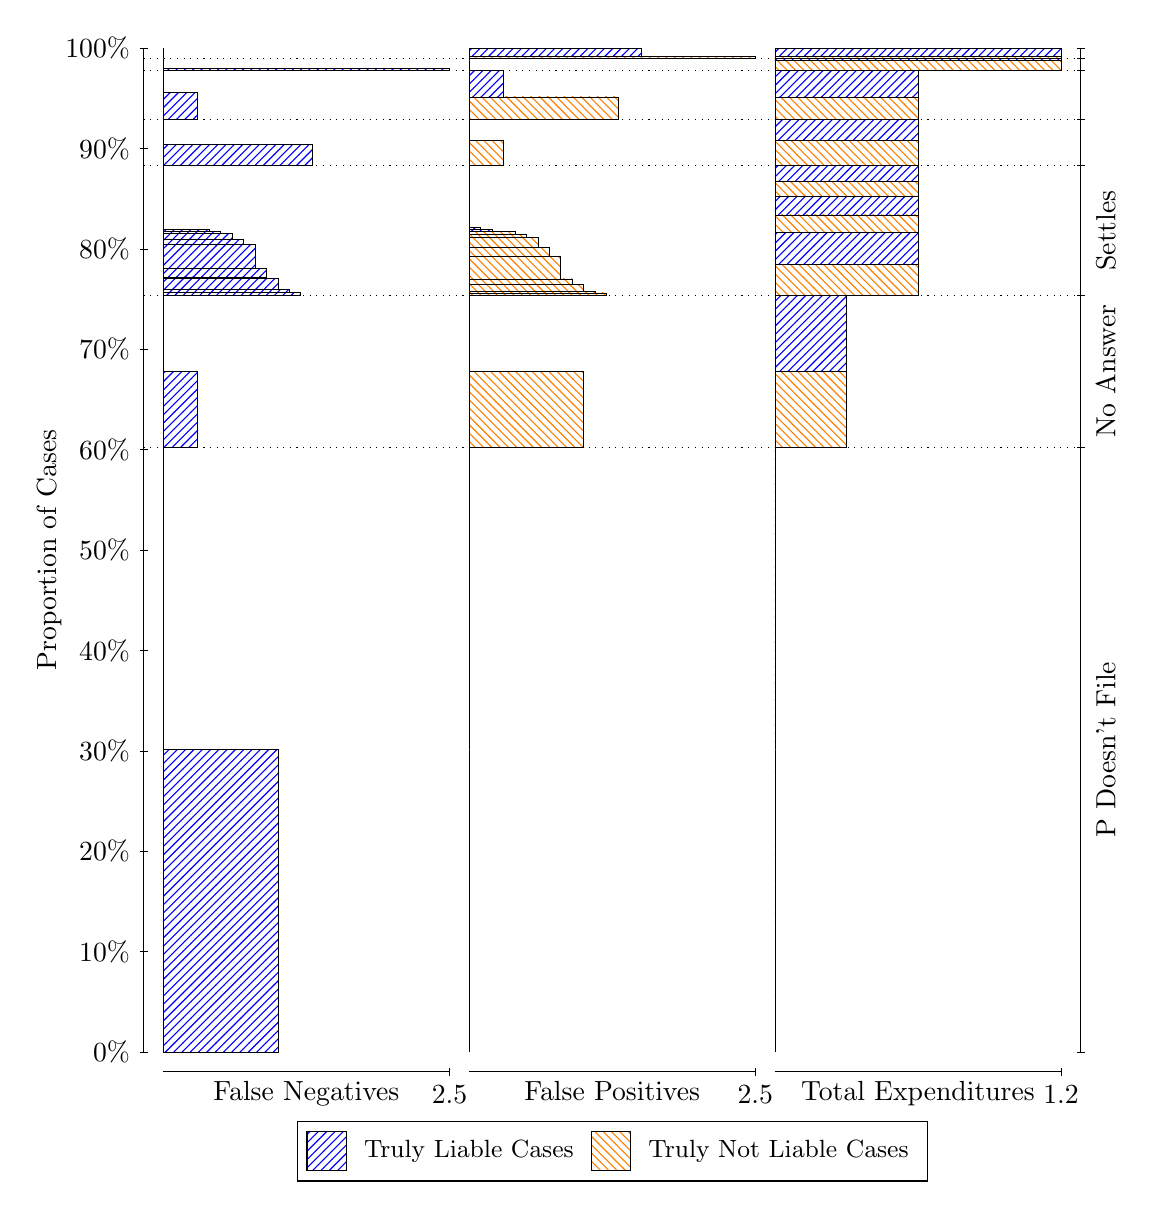
\begin{tikzpicture}
\draw[black, very thin] (1.5,1.75) -- (1.5,14.5);
\node[rotate=90, anchor=center] at (0.3, 8.125) {Proportion of Cases};
\draw[black, very thin] (1.45,1.75) -- (1.55,1.75);
\node[anchor=east] at (1.45, 1.75) {0\%};
\draw[black, very thin] (1.45,3.025) -- (1.55,3.025);
\node[anchor=east] at (1.45, 3.025) {10\%};
\draw[black, very thin] (1.45,4.3) -- (1.55,4.3);
\node[anchor=east] at (1.45, 4.3) {20\%};
\draw[black, very thin] (1.45,5.575) -- (1.55,5.575);
\node[anchor=east] at (1.45, 5.575) {30\%};
\draw[black, very thin] (1.45,6.85) -- (1.55,6.85);
\node[anchor=east] at (1.45, 6.85) {40\%};
\draw[black, very thin] (1.45,8.125) -- (1.55,8.125);
\node[anchor=east] at (1.45, 8.125) {50\%};
\draw[black, very thin] (1.45,9.4) -- (1.55,9.4);
\node[anchor=east] at (1.45, 9.4) {60\%};
\draw[black, very thin] (1.45,10.675) -- (1.55,10.675);
\node[anchor=east] at (1.45, 10.675) {70\%};
\draw[black, very thin] (1.45,11.95) -- (1.55,11.95);
\node[anchor=east] at (1.45, 11.95) {80\%};
\draw[black, very thin] (1.45,13.225) -- (1.55,13.225);
\node[anchor=east] at (1.45, 13.225) {90\%};
\draw[black, very thin] (1.45,14.5) -- (1.55,14.5);
\node[anchor=east] at (1.45, 14.5) {100\%};

\draw[black, very thin] (13.4,1.75) -- (13.4,14.5);
\draw[black, very thin] (13.35,1.75) -- (13.45,1.75);
\node[anchor=west] at (13.35, 1.75) {};
\draw[black, very thin] (13.35,9.4299) -- (13.45,9.4299);
\node[anchor=west] at (13.35, 9.4299) {};
\draw[black, very thin] (13.35,11.36) -- (13.45,11.36);
\node[anchor=west] at (13.35, 11.36) {};
\draw[black, very thin] (13.35,13.008) -- (13.45,13.008);
\node[anchor=west] at (13.35, 13.008) {};
\draw[black, very thin] (13.35,13.593) -- (13.45,13.593);
\node[anchor=west] at (13.35, 13.593) {};
\draw[black, very thin] (13.35,14.22) -- (13.45,14.22);
\node[anchor=west] at (13.35, 14.22) {};
\draw[black, very thin] (13.35,14.37) -- (13.45,14.37);
\node[anchor=west] at (13.35, 14.37) {};
\draw[black, very thin] (13.35,14.5) -- (13.45,14.5);
\node[anchor=west] at (13.35, 14.5) {};

\draw[black, very thin, pattern color=blue, pattern=north east lines] (1.75,1.75) rectangle (3.2033,5.5899);
\draw[black, very thin, pattern color=orange, pattern=north west lines] (1.75,5.5899) rectangle (1.75,9.4299);
\draw[black, very thin, pattern color=blue, pattern=north east lines] (1.75,9.4299) rectangle (2.186,10.395);
\draw[black, very thin, pattern color=orange, pattern=north west lines] (1.75,10.395) rectangle (1.75,11.36);
\draw[black, very thin, pattern color=blue, pattern=north east lines] (1.75,11.36) rectangle (3.494,11.395);
\draw[black, very thin, pattern color=blue, pattern=north east lines] (1.75,11.395) rectangle (3.3487,11.43);
\draw[black, very thin, pattern color=blue, pattern=north east lines] (1.75,11.43) rectangle (3.2033,11.574);
\draw[black, very thin, pattern color=blue, pattern=north east lines] (1.75,11.574) rectangle (3.058,11.593);
\draw[black, very thin, pattern color=blue, pattern=north east lines] (1.75,11.593) rectangle (3.058,11.704);
\draw[black, very thin, pattern color=blue, pattern=north east lines] (1.75,11.704) rectangle (2.9127,12.008);
\draw[black, very thin, pattern color=blue, pattern=north east lines] (1.75,12.008) rectangle (2.7673,12.073);
\draw[black, very thin, pattern color=blue, pattern=north east lines] (1.75,12.073) rectangle (2.622,12.144);
\draw[black, very thin, pattern color=blue, pattern=north east lines] (1.75,12.144) rectangle (2.4767,12.17);
\draw[black, very thin, pattern color=blue, pattern=north east lines] (1.75,12.17) rectangle (2.3313,12.196);
\draw[black, very thin, pattern color=orange, pattern=north west lines] (1.75,12.196) rectangle (1.75,13.008);
\draw[black, very thin, pattern color=blue, pattern=north east lines] (1.75,13.008) rectangle (3.6393,13.272);
\draw[black, very thin, pattern color=orange, pattern=north west lines] (1.75,13.272) rectangle (1.75,13.593);
\draw[black, very thin, pattern color=blue, pattern=north east lines] (1.75,13.593) rectangle (2.186,13.932);
\draw[black, very thin, pattern color=orange, pattern=north west lines] (1.75,13.932) rectangle (1.75,14.22);
\draw[black, very thin, pattern color=blue, pattern=north east lines] (1.75,14.22) rectangle (5.3833,14.246);
\draw[black, very thin, pattern color=orange, pattern=north west lines] (1.75,14.246) rectangle (1.75,14.37);
\draw[black, very thin, pattern color=orange, pattern=north west lines] (1.75,14.37) rectangle (1.75,14.397);
\draw[black, very thin, pattern color=blue, pattern=north east lines] (1.75,14.397) rectangle (1.75,14.5);
\draw[black, very thin, pattern color=orange, pattern=north west lines] (5.6333,1.75) rectangle (5.6333,5.59);
\draw[black, very thin, pattern color=blue, pattern=north east lines] (5.6333,5.59) rectangle (5.6333,9.4299);
\draw[black, very thin, pattern color=orange, pattern=north west lines] (5.6333,9.4299) rectangle (7.0867,10.395);
\draw[black, very thin, pattern color=blue, pattern=north east lines] (5.6333,10.395) rectangle (5.6333,11.36);
\draw[black, very thin, pattern color=orange, pattern=north west lines] (5.6333,11.36) rectangle (7.3773,11.389);
\draw[black, very thin, pattern color=orange, pattern=north west lines] (5.6333,11.389) rectangle (7.232,11.414);
\draw[black, very thin, pattern color=orange, pattern=north west lines] (5.6333,11.414) rectangle (7.0867,11.494);
\draw[black, very thin, pattern color=orange, pattern=north west lines] (5.6333,11.494) rectangle (6.9413,11.568);
\draw[black, very thin, pattern color=orange, pattern=north west lines] (5.6333,11.568) rectangle (6.796,11.858);
\draw[black, very thin, pattern color=orange, pattern=north west lines] (5.6333,11.858) rectangle (6.6507,11.968);
\draw[black, very thin, pattern color=orange, pattern=north west lines] (5.6333,11.968) rectangle (6.5053,12.095);
\draw[black, very thin, pattern color=orange, pattern=north west lines] (5.6333,12.095) rectangle (6.36,12.131);
\draw[black, very thin, pattern color=orange, pattern=north west lines] (5.6333,12.131) rectangle (6.2147,12.171);
\draw[black, very thin, pattern color=blue, pattern=north east lines] (5.6333,12.171) rectangle (5.924,12.198);
\draw[black, very thin, pattern color=blue, pattern=north east lines] (5.6333,12.198) rectangle (5.7787,12.223);
\draw[black, very thin, pattern color=blue, pattern=north east lines] (5.6333,12.223) rectangle (5.6333,13.008);
\draw[black, very thin, pattern color=orange, pattern=north west lines] (5.6333,13.008) rectangle (6.0693,13.329);
\draw[black, very thin, pattern color=blue, pattern=north east lines] (5.6333,13.329) rectangle (5.6333,13.593);
\draw[black, very thin, pattern color=orange, pattern=north west lines] (5.6333,13.593) rectangle (7.5227,13.88);
\draw[black, very thin, pattern color=blue, pattern=north east lines] (5.6333,13.88) rectangle (6.0693,14.22);
\draw[black, very thin, pattern color=orange, pattern=north west lines] (5.6333,14.22) rectangle (5.6333,14.343);
\draw[black, very thin, pattern color=blue, pattern=north east lines] (5.6333,14.343) rectangle (5.6333,14.37);
\draw[black, very thin, pattern color=orange, pattern=north west lines] (5.6333,14.37) rectangle (9.2667,14.397);
\draw[black, very thin, pattern color=blue, pattern=north east lines] (5.6333,14.397) rectangle (7.8133,14.5);
\draw[black, very thin, pattern color=orange, pattern=north west lines] (9.5167,1.75) rectangle (9.5167,5.59);
\draw[black, very thin, pattern color=blue, pattern=north east lines] (9.5167,5.59) rectangle (9.5167,9.4299);
\draw[black, very thin, pattern color=orange, pattern=north west lines] (9.5167,9.4299) rectangle (10.425,10.395);
\draw[black, very thin, pattern color=blue, pattern=north east lines] (9.5167,10.395) rectangle (10.425,11.36);
\draw[black, very thin, pattern color=orange, pattern=north west lines] (9.5167,11.36) rectangle (11.333,11.756);
\draw[black, very thin, pattern color=blue, pattern=north east lines] (9.5167,11.756) rectangle (11.333,12.158);
\draw[black, very thin, pattern color=orange, pattern=north west lines] (9.5167,12.158) rectangle (11.333,12.38);
\draw[black, very thin, pattern color=blue, pattern=north east lines] (9.5167,12.38) rectangle (11.333,12.613);
\draw[black, very thin, pattern color=orange, pattern=north west lines] (9.5167,12.613) rectangle (11.333,12.806);
\draw[black, very thin, pattern color=blue, pattern=north east lines] (9.5167,12.806) rectangle (11.333,13.008);
\draw[black, very thin, pattern color=orange, pattern=north west lines] (9.5167,13.008) rectangle (11.333,13.329);
\draw[black, very thin, pattern color=blue, pattern=north east lines] (9.5167,13.329) rectangle (11.333,13.593);
\draw[black, very thin, pattern color=orange, pattern=north west lines] (9.5167,13.593) rectangle (11.333,13.88);
\draw[black, very thin, pattern color=blue, pattern=north east lines] (9.5167,13.88) rectangle (11.333,14.22);
\draw[black, very thin, pattern color=orange, pattern=north west lines] (9.5167,14.22) rectangle (13.15,14.343);
\draw[black, very thin, pattern color=blue, pattern=north east lines] (9.5167,14.343) rectangle (13.15,14.37);
\draw[black, very thin, pattern color=orange, pattern=north west lines] (9.5167,14.37) rectangle (13.15,14.397);
\draw[black, very thin, pattern color=blue, pattern=north east lines] (9.5167,14.397) rectangle (13.15,14.5);
\draw[black, dotted] (1.5,9.4299) -- (13.4,9.4299);
\draw[black, dotted] (1.5,11.36) -- (13.4,11.36);
\draw[black, dotted] (1.5,13.008) -- (13.4,13.008);
\draw[black, dotted] (1.5,13.593) -- (13.4,13.593);
\draw[black, dotted] (1.5,14.22) -- (13.4,14.22);
\draw[black, dotted] (1.5,14.37) -- (13.4,14.37);
\draw[black, very thin] (1.75,1.5) -- (5.3833,1.5);
\node[anchor=north] at (3.5667, 1.5) {False Negatives};
\draw[black, very thin] (5.3833,1.45) -- (5.3833,1.55);
\node[anchor=north] at (5.3833, 1.45) {2.5};

\draw[black, very thin] (5.6333,1.5) -- (9.2667,1.5);
\node[anchor=north] at (7.45, 1.5) {False Positives};
\draw[black, very thin] (9.2667,1.45) -- (9.2667,1.55);
\node[anchor=north] at (9.2667, 1.45) {2.5};

\draw[black, very thin] (9.5167,1.5) -- (13.15,1.5);
\node[anchor=north] at (11.333, 1.5) {Total Expenditures};
\draw[black, very thin] (13.15,1.45) -- (13.15,1.55);
\node[anchor=north] at (13.15, 1.45) {1.2};

\node[black, centered, rotate=90] at (13.72, 5.59) {P Doesn't File};
\node[black, centered, rotate=90] at (13.72, 10.395) {No Answer};
\node[black, centered, rotate=90] at (13.72, 12.184) {Settles};





\draw (7.449999999999999,1.5) node[draw=none] (baseCoordinate) {};
\begin{scope}[align=center]
        \matrix[scale=0.5, draw=black, below=0.5cm of baseCoordinate, nodes={draw}, column sep=0.1cm]{
            \node[rectangle, draw, minimum width=0.5cm, minimum height=0.5cm, pattern=north east lines, pattern color=blue] {}; &
            \node[draw=none, font=\small] (B) {Truly Liable Cases}; &
            \node[rectangle, draw, minimum width=0.5cm, minimum height=0.5cm, pattern=north west lines, pattern color=orange] {}; &
            \node[draw=none, font=\small] (B) {Truly Not Liable Cases}; \\
            };
\end{scope}

\end{tikzpicture}
\end{document}